\subsection{Erzwungene Schwingungen}
\begin{frame}
\frametitle{Erzwungene Schwingungen, {\normalsize ungedämpft 1/3}}
\begin{columns}
        \begin{column}[t]{.5\linewidth}
\begin{figure}
         \begin{tikzpicture}[scale=0.6]
 \fill[black!5!white] (-1,-2) rectangle (7, 3); 
\draw[->] (2.5, 2) --(4, 2);
\draw (2.5,1.8) -- (2.5, 2.2);
\draw[thin] (4,1.5)--(4,2.2);
\draw (0, 0) pic [scale=0.6] {DKbase};
\draw (0, 0) pic [scale=0.6, thick] {DKspring=4};  
\draw[thick] (4,-1.5) rectangle +(1.5, 3); 
\draw (2, -0.9) node {$k$};
\draw (4.7, 0) node {$m$};
\draw (3.25, 2.3) node {$u$};
\draw[->, very thick] (5.7, 0) -- (6.9, 0);
\draw (6.25, 0.55) node {$F(t)$};
\end{tikzpicture}

        \uncover<2-4>{
        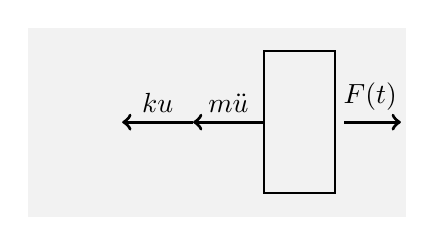
\begin{tikzpicture}[scale=0.6]
\fill[black!5!white] (-1,-2) rectangle (7, 2); 
\draw[thick] (4,-1.5) rectangle +(1.5, 3); 
\draw (3.25, 0.4) node {$m\ddot{u}$};
\draw (1.75, 0.4) node {$ku$};
\draw[<-, very thick] (2.5, 0) -- (4, 0);
\draw[<-, very thick] (1, 0) -- (2.5, 0);
\draw[->, very thick] (5.7, 0) -- (6.9, 0);
\draw (6.25, 0.55) node {$F(t)$};
\end{tikzpicture}

        }
        \caption*{Modell \uncover<2-4>{und Freischnitt}}
\end{figure}
        \end{column}
		\hfill
		\begin{column}[t]{.5\linewidth}
\uncover<3-4>{
		Bewegungsgleichung
\begin{equation*}
 F(t)-ku-m\ddot{u}=0
\end{equation*}
}
\uncover<4>{
Standardform
\begin{align*}
 \ddot{u}+\omega_0^2 u&=\omega_0^2 a(t)\\
 \omega_0^2&=\frac{k}{m}\\
 a(t)&= \frac{F(t)}{k}
\end{align*}
}
		\end{column}
\end{columns}
\end{frame}

\begin{frame}
\frametitle{Erzwungene Schwingungen, {\normalsize ungedämpft 2/3}}
\uncover<1-2>{
Die Gesamtlösung ist die Summe der Lösung der homogenen Gleichung (\textsl{Einschwingen}) und einer partikulären Lösung (\textsl{eingeschwungener Zustand})}
\begin{equation*}
 u(t)=u_h(t)+u_p(t).
\end{equation*}
Die Lösung der homogenen Gleichung entspricht der freien Schwingung. Um eine partikuläre Lösung für harmonische Anregung $F(t)=F_C\cos\omega t\uncover<1>{+F_S\sin\omega t}$ zu finden, wählen wir einen Ansatz vom Typ der rechten Seite
\begin{align*}
u_p(t)&=u_C\cos\omega t\uncover<1>{+u_S\sin\omega t},\\
\dot{u}_p(t)&=-u_C\omega\sin\omega t\uncover<1>{+u_S\omega\cos\omega t},\\
\ddot{u}_p(t)&=-u_C\omega^2\cos\omega t\uncover<1>{-u_S\omega^2\sin\omega t}.\\
\end{align*}
\uncover<2>{
Zunächst beschränken wir uns auf den Cosinus-Anteil (Sinus analog).}
\end{frame}


\begin{frame}
\frametitle{Erzwungene Schwingungen, {\normalsize ungedämpft 3/3}} 
\uncover<1-2>{
Einsetzen in die Bewegungsgleichung (Standardform) führt auf
\begin{equation*}
-u_C\omega^2\cos\omega t + u_C\omega_0^2\cos\omega t = a_C\omega_0^2\cos\omega t.
\end{equation*}
Koeffizientenvergleich liefert
\begin{equation*}
 u_C=\frac{\omega_0^2}{\omega_0^2-\omega^2}a_C
\quad \leadsto \quad 
 u_p(t)=\frac{1}{1-(\omega/\omega_0)^2}a_C \cos\omega t.
\end{equation*}
}
\uncover<2>{
Bei Resonanzanregung $\omega=\omega_0$ versagt dieser Ansatz, dann lautet die Lösung
\begin{equation*}
u_p(t)=\frac{\omega t}{2}\sin\omega t
\end{equation*}
Knobelspaß, siehe \textsl{Variation der Konstanten}!
}
\end{frame}


\begin{frame}
\frametitle{Erzwungene Schwingungen, {\normalsize gedämpft 1/5}}

\begin{columns}
        \begin{column}[t]{.5\linewidth}
        \begin{figure}
\begin{tikzpicture}[scale=0.6]
\fill[black!5!white] (-1,-3) rectangle (7, 3); 
\draw (0, 0) pic [scale=0.6] {DKbase};
\draw (0, 1) pic [scale=0.6, thick] {DKspring=4};
\draw (0,-1) pic [scale=0.6, thick] {DKdashpot=4};  
\draw[->] (2.5, 2) --(4, 2);
\draw (2.5,1.8) -- (2.5, 2.2);
\draw[thin] (4,1.5)--(4,2.2);
\draw[thick] (4,-1.5) rectangle +(1.5, 3); 
\draw (2.0, 0.1) node {$k$};
\draw (2.0,-1.9) node {$c$};
\draw (4.7, 0) node {$m$};
\draw (3.25, 2.3) node {$u$};
\draw[->, very thick] (5.7, 0) -- (6.9, 0);
\draw (6.25, 0.55) node {$F(t)$};
\end{tikzpicture}


\uncover<2-4>{
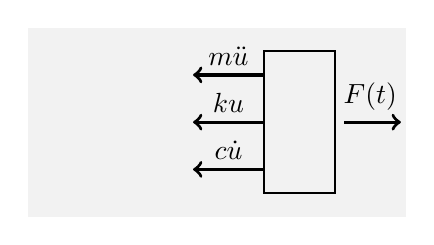
\begin{tikzpicture}[scale=0.6]
\fill[black!5!white] (-1,-2) rectangle (7, 2); 
\draw[thick] (4,-1.5) rectangle +(1.5, 3); 
\draw (3.25, 1.4) node {$m\ddot{u}$};
\draw (3.25, 0.4) node {$ku$};
\draw (3.25,-0.6) node {$c\dot{u}$};
\draw[<-, very thick] (2.5, 1) -- (4, 1);
\draw[<-, very thick] (2.5, 0) -- (4, 0);
\draw[<-, very thick] (2.5,-1) -- (4,-1);
\draw[->, very thick] (5.7, 0) -- (6.9, 0);
\draw (6.25, 0.55) node {$F(t)$};
\end{tikzpicture}

}
\caption*{Modell \uncover<2-4>{und Freischnitt}}
\end{figure}
        \end{column}
		\hfill
		\begin{column}[t]{.5\linewidth}
\uncover<3-4>{
		Bewegungsgleichung
\begin{equation*}
 F(t)-ku-c\dot{u}-m\ddot{u}=0
\end{equation*}
}
\uncover<4>{
Standardform
\begin{align*}
 \ddot{u}+2 \zeta\omega_0\dot{u}+\omega_0^2 u&=\omega_0^2 a(t)\\
 2 \zeta\omega_0&=\frac{c}{m}\\
 \omega_0^2&=\frac{k}{m}\\
  a(t)&= \frac{F(t)}{k}
\end{align*}
}
\end{column}
\end{columns}
\end{frame}


\begin{frame}
\frametitle{Erzwungene Schwingungen, {\normalsize gedämpft 2/5}}
Wie im ungedämpften Fall, und allgemein für jede inhomogene Differentialgleichung, gilt für die Gesamtlösung
\begin{equation*}
 u(t)=u_h(t)+u_p(t).
\end{equation*}
Für einfache harmonische Anregung $a(t)=a_C\cos\omega t + a_S \sin \omega t$
führt der Ansatz $u_p(t)=u_C\cos\omega t + u_S\sin\omega t$ auf
\begin{align*}
u_C&= V^2 \Bigl( (1-\eta^2)a_C-2\zeta\eta a_S \Bigl)\\
u_S&= V^2 \Bigl( (1-\eta^2)a_S+2\zeta\eta a_C \Bigl)
\end{align*}
Vergrößerungsfunktion $V=\frac{1}{\sqrt{(1-\eta^2)^2+(2\zeta\eta)^2}}$, \hfill Abstimmungsverhältnis $\eta= \frac{\omega}{\omega_0}$.
\smallskip
\begin{center}
 \textbf{Anmerkung:} der eingeschwungene Zustand für andere Anregungsarten (Dämpferfußpunkt-, Fundament-, Unwucht-) weist qualitative Unterschiede auf, die Herleitung verläuft aber analog.
\end{center}
\end{frame}

\begin{frame}
\frametitle{Erzwungene Schwingungen, {\normalsize gedämpft 3/5}}
Summen von Sinus- und Cosinusfunktionen lassen sich mittels
Additionstheoremen durch eine der beiden Funktionen darstellen
\begin{align*}
a(t)&= \hat{a}\cos(\omega t - \psi_a) = 
 \overbrace{\hat{a}\cos\psi_a}^{a_C} \cos(\omega t) +
 \overbrace{\hat{a}\sin\psi_a}^{a_S} \sin(\omega t).%\\
%u_p(t)&= \hat{u}\cos(\omega t - \psi_u) = 
% \hat{u}\cos\psi_u \cos(\omega t) +
% \hat{u}\sin\psi_u \sin(\omega t).
 \end{align*}
 Amplitude $\hat{a}$ und Phasenwinkel $\psi_a$ sind folglich festgelegt durch
 \begin{equation*}
  \hat{a}^2 = a_S^2+a_C^2 \qquad \text{und} \qquad
  \tan\psi_a = \frac{a_S}{a_C}. 
\end{equation*}
In dieser Darstellung lauten die Beziehungen zwischen Anregung und Antwort
\begin{equation*}
\frac{\hat{u}}{\hat{a}}=V \qquad \text{und} \qquad
\psi=\psi_u -\psi_a =  \arctan \left(\frac{2\zeta\eta}{1-\eta^2}\right).
\end{equation*}

Anmerkung: Die Phasendifferenz wird üblicherweise auf $\psi\in(-\pi,\pi]$ begrenzt.
\end{frame}


\begin{frame}
\frametitle{Erzwungene Schwingungen, {\normalsize gedämpft 4/5}}

\only<1>{
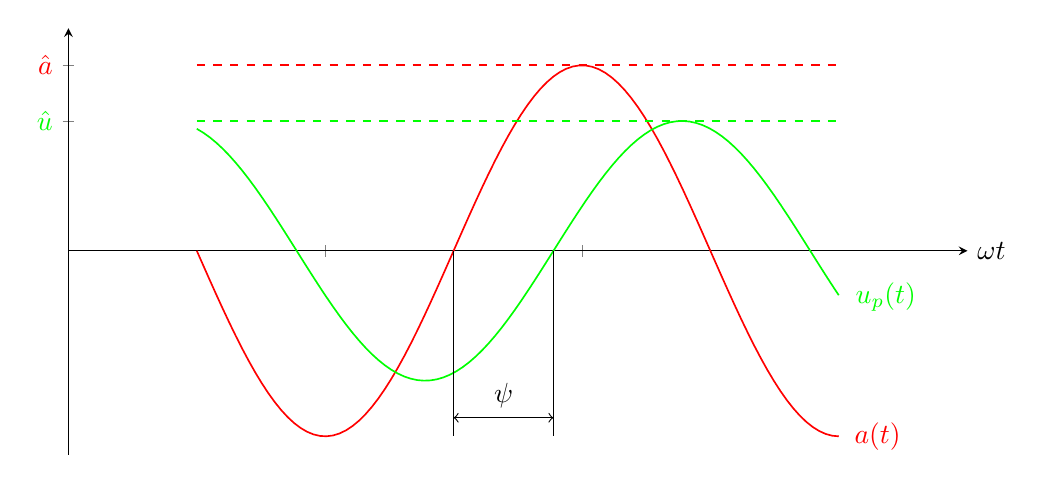
\begin{tikzpicture}
\begin{axis}[
    width=13cm, 
    height=7cm,
    axis x line=center, 
    axis y line=middle, 
    xlabel={$\omega t$},
     x label style={at={(current axis.right of origin)}, right},
    samples=100,
    ymin=-1.1, ymax=1.2,
    xmin=0, xmax=11,
    domain=0.5*pi:3*pi,
    xtick={   3.14159,  6.28318  },
    xticklabels={  ,  }, 
    ytick={0.7, 1},
    yticklabels={{\color{green}$\hat{u}$}, {\color{red} $\hat{a}$}}
]
\addplot [mark=none, semithick, red, dashed] {1};
\addplot [mark=none, semithick, red] {cos(deg(x))};
\addplot [mark=none, semithick, green, dashed] {0.7};
\addplot [mark=none, semithick, green] {0.7*cos(deg(x)-70)};
\node[text=red] at (axis cs: 9.9,-1.0) {$a(t)$};
\node[text=green] at (axis cs:10.0,-0.25) {$u_p(t)$};
\draw (axis cs: 4.712389, 0) -- (axis cs: 4.712389, -1);
\draw (axis cs: 5.934119, 0) -- (axis cs: 5.934119, -1);
\draw[<->] (axis cs: 4.712389, -0.9) -- node[above]{$\psi$} (axis cs: 5.934119, -0.9);
\end{axis}
\end{tikzpicture}

}

\only<2>{
\begin{figure}
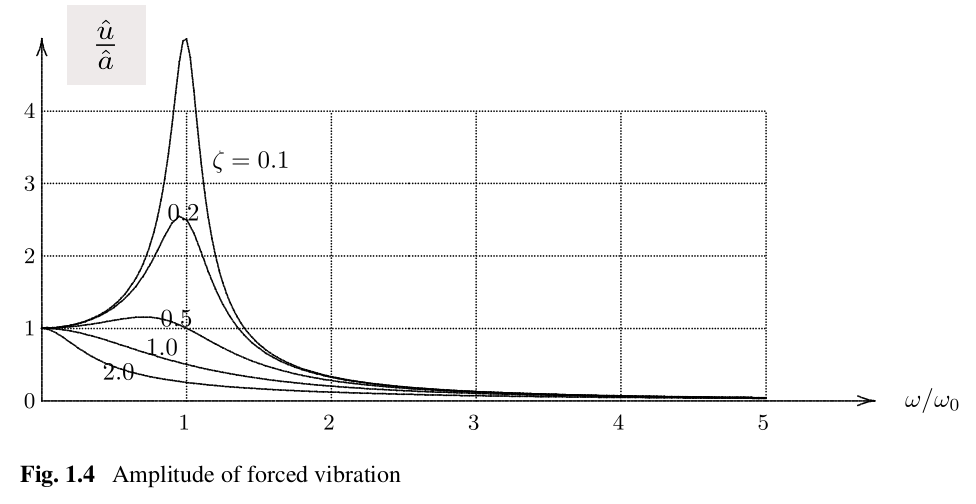
\includegraphics[width=0.9\textwidth]{fig_img/magnitude_response.png}
\caption*{aus \cite{Verruijt2010}}
\end{figure}
}

\only<3>{
\begin{figure}
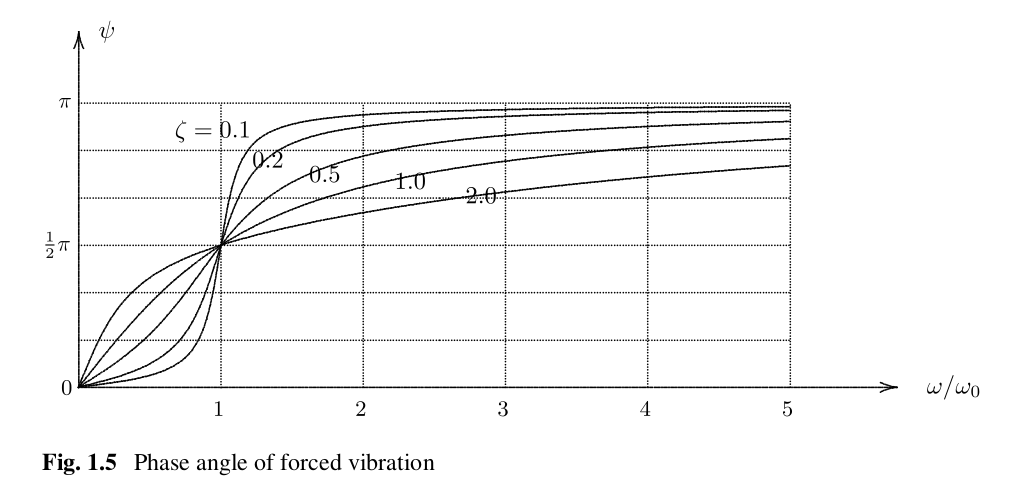
\includegraphics[width=\textwidth]{fig_img/phase_response.png}
\caption*{aus \cite{Verruijt2010}}
\end{figure}
}

\end{frame}

\begin{frame}
\frametitle{Erzwungene Schwingungen, {\normalsize gedämpft 5/5}}
Die Gesamtlösung lautet
\begin{equation*}
 u(t)=e^{-\delta t}\bigl( C_1\cos\omega_1 t + C_2\sin\omega_1 t \bigr)
 +u_C\cos\omega t + u_S\sin\omega t,
\end{equation*}
die unbestimmten Koeffizienten $C_1$ und $C_2$ folgen aus den Anfangsbedingungen
\begin{align*}
 u(t_0)&=u_0,\\
 \dot{u}(t_0)&=\dot{u}_0.
\end{align*}
\end{frame}
